% =========================================================================
% Budget-Constrained Confidence Ranking for Black-Box LLMs
% Methodology (Sec. 3) and Experimental Setup (Sec. 4) -- working draft v2
%
% Compiles standalone with pdflatex. To target a venue, replace the
% \documentclass and preamble with the venue style (e.g. acl.sty for
% *ACL industry track, icml/neurips styles) -- section bodies, theorem
% environments and macros below are style-agnostic.
%
% v2: adds Lemmas 2-4, Proposition 2 (elevated), Corollary 1
% (certification depth), Proposition 3 (evidence exchange) with the
% evidence-equivalence experiment arm; corrects numerical constants
% (all verified computationally); Miller-Madow-corrected entropy;
% per-batch strata, held-out probe execution scope, distractor-pool
% disjointness, and the operational evaluation conventions.
% =========================================================================
\documentclass[11pt]{article}

\usepackage[margin=1in]{geometry}
\usepackage{amsmath,amssymb,amsthm}
\usepackage{booktabs}
\usepackage{graphicx}
\usepackage{pifont}
\usepackage{array}
\usepackage{enumitem}
\usepackage{microtype}
\usepackage[colorlinks=true,linkcolor=blue,citecolor=blue,urlcolor=blue]{hyperref}
\usepackage[round]{natbib}

% ----- theorem environments ---------------------------------------------
\newtheorem{assumption}{Assumption}
\newtheorem{proposition}{Proposition}
\newtheorem{lemma}{Lemma}
\newtheorem{corollary}{Corollary}
\newtheorem{remark}{Remark}

% ----- notation macros ---------------------------------------------------
\newcommand{\pbar}{\bar{p}}
\newcommand{\E}{\mathbb{E}}
\newcommand{\Prob}{\mathbb{P}}
\newcommand{\ind}{\mathbf{1}}
\newcommand{\Bern}{\mathrm{Bern}}
\newcommand{\Betadist}{\mathrm{Beta}}
\newcommand{\SE}{\mathrm{SE}}
\newcommand{\score}{s}
\newcommand{\sigsetX}{\mathcal{S}}
\newcommand{\precat}[1]{\mathrm{prec}@#1}
\newcommand{\keff}{k_{\mathrm{eff}}}

\title{Budget-Constrained Confidence Ranking for Black-Box LLMs:\\
Label-Free Top-$k$ Selection with Sequential Sampling Guarantees\\
{\large --- Methodology and Experimental Setup (working draft v2) ---}}
\author{}
\date{}

\begin{document}
\maketitle

% =========================================================================
\section{Methodology}
\label{sec:method}
% =========================================================================

\begin{figure}[t]
  \centering
  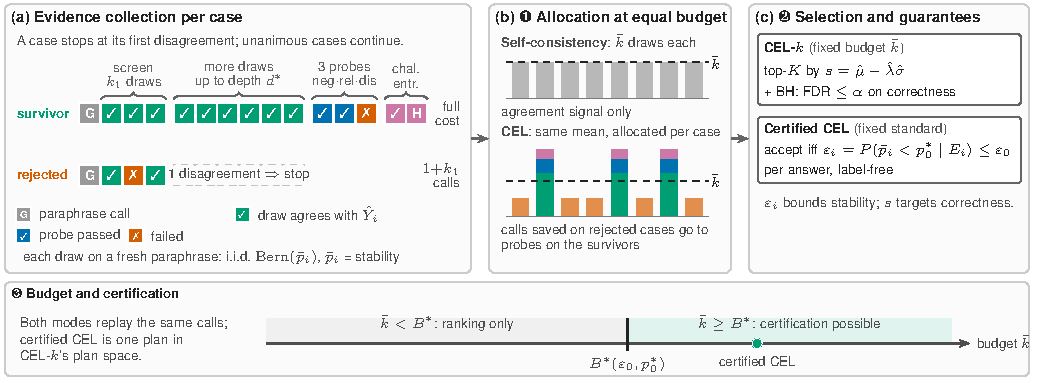
\includegraphics[width=\textwidth]{figures/fig1_overview.pdf}
  \caption{\textbf{Overview of CEL.}
  (a)~Each case is screened with $k_1$ draws on fresh paraphrases; one
  disagreement with the majority answer ends it at $1 + k_1$ calls. Only
  unanimous cases buy more evidence: draws up to depth $d^\ast$, the probes,
  the challenge and the entropy call.
  (b)~\ding{182}~At the same mean budget $\bar k$,
  self-consistency spends every call on draws, which cannot see a
  stable-but-wrong answer. CEL spends little on rejected cases and uses
  the saved calls for probes on the survivors.
  (c)~\ding{183}~Fixing the budget gives a
  ranking by the fitted score $s$ (model-based), with an exact FDR bound on
  correctness from conformal BH on a labelled calibration split. Fixing an
  evidence standard $(\varepsilon_0, p_0^\ast)$, chosen by the user, gives
  an exact, label-free certificate of stability for each accepted answer.
  \ding{184}~Both modes replay the same calls. Below the
  certification budget $B^\ast$ (Cor.~\ref{cor:certbudget}) CEL-$k$ can rank
  but not certify, and certified CEL is one plan in CEL-$k$'s plan space
  (Prop.~\ref{prop:nesting}). The depth $d^\ast$ and $B^\ast$ follow from
  the standard. Our experiments use $k_1 = 3$ and
  $(\varepsilon_0, p_0^\ast) = (0.05, 0.8)$, giving $d^\ast = 9$ and $4$ or
  $15$ calls per case; the bars in (b) are illustrative.}
  \label{fig:overview}
\end{figure}

\subsection{Problem Formulation and Selection Optimality}
\label{sec:method:setup}

Let $f$ denote a black-box LLM accessible only through sampled responses:
no token-level probabilities, no gradients, no training access. Let
$\{x_i\}_{i=1}^{N}$ be a batch of binary questions, and let $B$ be a total
API-call budget for the batch. For case $i$ and prompt phrasing $j$, let
$p_{ij}$ denote the probability that $f$ emits case $i$'s majority answer
under phrasing $j$ at fixed decoding parameters. Because confidence should
not be an artifact of one phrasing, the target of inference is the
\emph{phrasing-marginal stability}
\begin{equation}
  \pbar_i \;=\; \E_{J \sim Q}\!\left[p_{iJ}\right],
  \label{eq:pbar}
\end{equation}
where $Q$ is a distribution over semantics-preserving paraphrases of
$x_i$. The task is to select a subset $T \subset \{1,\dots,N\}$ with
$|T| = k$ (here the top $10\%$ of the batch, $k = 5$ of $N = 50$) maximizing the expected number of correct
answers $\E\!\left[\#\text{correct in } T\right]$, subject to total spend
at most $B$, \emph{without labels}.

Every quantity we estimate is behavioral; a single explicitly stated
assumption bridges behavior to correctness. Writing $\hat Y_i$ for the
majority answer and $Z_i = \ind\{\hat Y_i = Y_i\}$ for its correctness,
the composite score $\score_i$ of Section~\ref{sec:method:agg} is a
predictor of $Z_i$, and:

\begin{assumption}[Monotonicity]
\label{ass:mono}
The conditional accuracy
$\pi(\score) = \Prob(Z = 1 \mid \score)$ is nondecreasing in $\score$.
\end{assumption}

\begin{proposition}[Optimality of top-$k$ selection]
\label{prop:topk}
Under Assumption~\ref{ass:mono}, the rule ``select the $k$ cases with the
largest $\score_i$'' maximizes $\E\!\left[\#\mathrm{correct\ in\ }
T\right]$ over all size-$k$ selection rules.
\end{proposition}

\begin{proof}
By linearity of expectation (no cross-case independence is required),
$\E[\#\text{correct in } T] = \sum_{i \in T} \pi(\score_i)$. Let $T$ be
any size-$k$ set that is not the top-$k$ by $\score$. Then there exist
$a \notin T$ and $b \in T$ with $\score_a > \score_b$. The swap
$T' = T \cup \{a\} \setminus \{b\}$ changes the objective by
$\pi(\score_a) - \pi(\score_b) \ge 0$ by Assumption~\ref{ass:mono}. Each
such swap strictly increases the number of top-$k$ members of the
selected set, so after at most $k$ swaps the top-$k$ set is reached with
the objective never decreased. Hence no size-$k$ set attains a strictly
larger objective.
\end{proof}

\begin{remark}
Proposition~\ref{prop:topk} is the Neyman--Pearson exchange argument
transplanted to selection: score plays the role of the likelihood ratio,
the selection size $k$ the role of the test size. It delivers optimality
\emph{given} the score and certifies that ranking-grade confidence is
sufficient --- no calibration ($\pi(\score) = \score$) is required,
which is what permits a label-free pipeline. It is silent on the quality
of the score itself, the subject of
Sections~\ref{sec:method:signals}--\ref{sec:method:shapley}.
Assumption~\ref{ass:mono} is not verifiable without labels;
Section~\ref{sec:exp} tests it empirically on labeled benchmarks,
globally (score-decile shape) and locally at the top of the ranking,
where the proposition consumes it.
\end{remark}

% -------------------------------------------------------------------------
\subsection{Budget-Optimal Sampling Design}
\label{sec:method:design}

\paragraph{Fresh-paraphrase sampling is exactly i.i.d.}
Repeated samples of a \emph{single} phrasing are conditionally correlated
through prompt-specific bias (wording effects, position effects), which
degrades the information per call. Our protocol removes this by design.

\begin{lemma}[Fresh-paraphrase i.i.d.\ sampling]
\label{lem:iid}
Fix a case and suppress its index. Suppose each draw $t = 1, 2, \dots$ is
generated by the two-stage mechanism $J_t \sim Q$ i.i.d., then
$Y_t \mid J_t \sim \Bern(p_{J_t})$, with the pairs $(J_t, Y_t)$
independent across $t$. Then $Y_1, Y_2, \dots$ are i.i.d.\
$\Bern(\pbar)$ with $\pbar = \E_{J\sim Q}[p_J]$.
\end{lemma}

\begin{proof}
Marginally, $\Prob(Y_t = 1) = \E_Q[p_{J_t}] = \pbar$ for every $t$, and
independence of the pairs across $t$ implies independence of the
$Y_t$. A mixture of Bernoullis is a Bernoulli at the mixture mean.
\end{proof}

Lemma~\ref{lem:iid} motivates the protocol used throughout: \emph{every
response draw uses a freshly sampled paraphrase, one draw per
paraphrase}. The cost of deviating from it is quantified by the
classical cluster-sampling penalty:

\begin{lemma}[Design effect of paraphrase reuse]
\label{lem:deff}
Allocate $n$ draws as $g$ paraphrases $\times$ $m = n/g$ draws each,
with per-draw marginal variance $\sigma^2 = \pbar(1-\pbar)$ and
within-paraphrase correlation $\rho \ge 0$. Then
\begin{equation}
  \mathrm{Var}\!\left(\hat{\pbar}\right)
  \;=\; \frac{\sigma^2}{n}\left[\,1 + (m - 1)\,\rho\,\right],
  \label{eq:deff}
\end{equation}
minimized over allocations at $m = 1$ (i.e.\ $g = n$), where the
bracket equals $1$.
\end{lemma}

\begin{proof}
$\mathrm{Var}(\sum_t Y_t) = n\sigma^2 + \sum_{t \neq t'}
\mathrm{Cov}(Y_t, Y_{t'})$. Covariances vanish across paraphrases and
equal $\rho\sigma^2$ within; there are $g\, m(m-1)$ ordered
within-paraphrase pairs, giving $n\sigma^2[1 + (m-1)\rho]$. Divide by
$n^2$. The bracket is increasing in $m$, hence minimized at $m=1$.
\end{proof}

Lemma~\ref{lem:iid} is the $m = 1$ corner of Lemma~\ref{lem:deff} at
which the i.i.d.\ description becomes exact rather than approximate;
the \emph{no-spread} ablation of Section~\ref{sec:exp:baselines}
measures the bracket of Eq.~\eqref{eq:deff} empirically. Two further
consequences: the posterior of Section~\ref{sec:method:posterior} is
exact, and the estimand is unambiguously $\pbar$ of Eq.~\eqref{eq:pbar}
\emph{relative to the paraphrase frame $Q$}. The latter is the honest
fine print: a paraphrase generator that drifts semantically does not
violate independence but \emph{contaminates the estimand}; we therefore
audit meaning preservation on a development slice
(Section~\ref{sec:exp:pipeline}).

\paragraph{Sequential triage via a truncated SPRT.}
Screening tests $H_0 : \pbar \le p_0$ against $H_1 : \pbar \ge p_1$
(we use $p_0 = 0.7$, $p_1 = 0.95$) on the i.i.d.\ agreement stream of
Lemma~\ref{lem:iid}. After $n$ draws with $S_n$ agreements, Wald's
sequential probability ratio test \citep{wald1945} tracks
\begin{equation}
  \Lambda_n \;=\; S_n \log\frac{p_1}{p_0}
  \;+\; (n - S_n)\log\frac{1 - p_1}{1 - p_0}
  \;\approx\; 0.305\, S_n \;-\; 1.792\,(n - S_n),
  \label{eq:sprt}
\end{equation}
stopping to accept $H_1$ when $\Lambda_n \ge A \approx
\log\frac{1-\beta}{\alpha}$ and to accept $H_0$ when $\Lambda_n \le
B_\ell \approx \log\frac{\beta}{1-\alpha}$; at $\alpha = \beta = 0.1$,
$A \approx 2.20$ and $B_\ell \approx -2.20$. By the Wald--Wolfowitz
theorem \citep{waldwolfowitz1948}, the SPRT minimizes the expected
number of draws under both hypotheses among all tests with the same
error rates. We truncate it into two stages:

\begin{itemize}[leftmargin=1.6em, itemsep=1pt]
\item \textbf{Stage 1 (screen):} $3$ draws; any disagreement
  $\Rightarrow$ eliminate. Since $3 \times 0.305 = 0.92 < A$, stage~1
  \emph{never certifies}: unanimous survivors occupy the SPRT's
  continuation region.
\item \textbf{Stage 2 (probe):} survivors receive $6$ further draws (the
  continuation of the same stream), alongside the orthogonal probes of
  Section~\ref{sec:method:signals}. Certification ($\Lambda \ge A$,
  i.e.\ $\approx 8$ net-clean agreements) can only complete here.
\end{itemize}

The two-stage pipeline is thus a single truncated SPRT with its
continuation region relabeled, not two ad hoc phases. Its economics are
exactly computable:

\begin{lemma}[Operating characteristics of the triage]
\label{lem:triage}
(a) The stage-1 screen passes a case with probability exactly
$\pbar^{\,3}$: $0.343$ at the $H_0$ boundary ($\pbar = 0.7$) and
$0.857$ at the $H_1$ boundary ($\pbar = 0.95$).
(b) Let $D(p) = p \log\frac{p_1}{p_0} + (1-p)\log\frac{1-p_1}{1-p_0}$
be the per-draw drift of $\Lambda_n$. Wald's identity
$\E[\Lambda_N] = \E[N]\, D(p)$ gives, with the boundary approximations,
\begin{equation}
  \E[N \mid H_0] \approx \frac{\alpha A + (1-\alpha) B_\ell}{D(p_0)}
  \approx \frac{-1.76}{-0.324} \approx 5.4,
  \qquad
  \E[N \mid H_1] \approx \frac{(1-\beta) A + \beta B_\ell}{D(p_1)}
  \approx \frac{1.76}{0.200} \approx 8.8,
  \label{eq:waldEN}
\end{equation}
versus $n \approx 12$ for a fixed-sample test at the same error rates
(normal approximation): sequential triage spends roughly $55\%$ fewer
draws on unstable cases and $27\%$ fewer on stable ones.
\end{lemma}

\begin{proof}
(a) is the probability of three successes in three i.i.d.\
$\Bern(\pbar)$ draws. (b) $\Lambda_N$ is a stopped random walk with
i.i.d.\ increments of mean $D(p)$; Wald's identity applies, and at
stopping $\Lambda_N$ sits approximately at a boundary, so
$\E[\Lambda_N]$ equals the acceptance-probability-weighted boundary
average; solve for $\E[N]$. The fixed-sample size follows from the
two-sided normal approximation
$n \ge \big(z_{1-\alpha}(\sigma_0 + \sigma_1)/(p_1 - p_0)\big)^2$.
\end{proof}

The step asymmetry in Eq.~\eqref{eq:sprt} --- one disagreement
($-1.79$) outweighs nearly six agreements ($+0.305$ each), and drift is
steeply negative under $H_0$ but shallow under $H_1$ --- makes
\emph{rejection cheap and certification expensive}, which is precisely
the economy a top-$k$ funnel requires: most cases need only
elimination-grade evidence. Stage-2 depth is fixed rather than adaptive
so that the entropy estimates of Section~\ref{sec:method:signals} share
comparable small-sample bias across cases; truncation of the joint
two-stage procedure slightly perturbs the nominal error rates relative
to Wald's bounds, quantified by simulation and reported with the
implementation (stage 1 alone is exact by Lemma~\ref{lem:triage}(a)).

% -------------------------------------------------------------------------
\subsection{Stability Posterior}
\label{sec:method:posterior}

Pooling a case's $k_i$ i.i.d.\ draws with $m_i$ agreements under the
Jeffreys prior $\Betadist(\tfrac12, \tfrac12)$ yields the posterior
\begin{equation}
  \pbar_i \mid \text{data} \;\sim\;
  \Betadist\!\left(m_i + \tfrac12,\; k_i - m_i + \tfrac12\right),
  \label{eq:posterior}
\end{equation}
exact under Lemma~\ref{lem:iid}. Two functionals are used downstream:
the \emph{lower credible bound} $L_i(\alpha) =
F^{-1}_{\pbar_i \mid \text{data}}(\alpha)$, which is the first
confidence signal and is budget-honest by construction (unanimity at
small $k_i$ yields only modest bounds), and the \emph{tail mass}
\begin{equation}
  \varepsilon_i \;=\; \Prob\!\left(\pbar_i < p_0^{\ast} \mid
  \text{data}\right)
  \;=\; F_{\Betadist(m_i + \frac12,\, k_i - m_i + \frac12)}(p_0^{\ast})
  \label{eq:eps}
\end{equation}
at a stability standard $p_0^{\ast}$ (we report $p_0^{\ast} = 0.8$),
which feeds the selection guarantee of
Section~\ref{sec:method:guarantee}. For calibration of intuition (all
values computed exactly): $9/9$ unanimous draws give $\varepsilon
\approx 0.042$; $12/12$ give $\varepsilon \approx 0.019$; a single
disagreement ($8/9$) gives $\varepsilon \approx 0.27$.

% -------------------------------------------------------------------------
\subsection{Signal Battery}
\label{sec:method:signals}

Stage-2 survivors are scored on five signals, listed in the prior
reliability order asserted by the cascade of
Section~\ref{sec:method:agg} (an assertion that the Shapley analysis of
Section~\ref{sec:method:shapley} tests rather than presumes).

\paragraph{(1) Agreement lower bound.} $L_i(\alpha)$ from
Eq.~\eqref{eq:posterior}.

\paragraph{(2) Invariance battery (specification test).}
Let $g$ be an input transformation with a known action $\sigma_g$ on the
correct label: logical negation ($\sigma_g(y) = 1 - y$), candidate or
option reordering (a relabeling), and insertion of an irrelevant
distractor ($\sigma_g = \mathrm{id}$). Define the consistency indicator
\begin{equation}
  C_i(g) \;=\; \ind\!\left\{\, f\!\left(g(x_i)\right) =
  \sigma_g\!\left(f(x_i)\right) \right\},
  \label{eq:flip}
\end{equation}
and the signal as the pass fraction over the battery. Its necessity is
an identifiability statement:

\begin{lemma}[Power separation]
\label{lem:power}
Let $H_{\mathrm{cue}}$ denote the alternative under which the model's
answer is a fixed function of a surface feature preserved by every
paraphrase in $Q$, and $H_{\mathrm{concept}}$ the hypothesis that the
model computes a function of the underlying proposition, answering
correctly under label-action transformations up to error $\epsilon$.
Then: (i) the resampled answer stream $\{Y_t\}$ of
Lemma~\ref{lem:iid} has the same law, $\Bern(\pbar)^{\otimes n}$, under
a stably wrong cue-follower as under a stably right concept-computer
with the same $\pbar$; hence any test observing only $\{Y_t\}$ has
power equal to its size against $H_{\mathrm{cue}}$. (ii) A battery of
$r$ label-action transformations that destroy or invert the cue
separates the hypotheses: the cue-follower passes all $r$ with
probability at most $(\tfrac12 + \delta)^{r}$ for binary answers,
while the concept-computer passes with probability at least
$(1-\epsilon)^{r}$.
\end{lemma}

\begin{proof}
(i) Both hypotheses induce i.i.d.\ $\Bern(\pbar)$ draws with the same
$\pbar$; identical laws yield identical rejection probabilities for any
measurable test, so power cannot exceed size. (ii) Under
$H_{\mathrm{cue}}$ the transformed input carries a destroyed or
inverted cue, making agreement with $\sigma_g(f(x))$ a
$\approx\!\tfrac12$-probability event per probe; independence across
probes gives the product bounds.
\end{proof}

Lemma~\ref{lem:power}(i) is why no amount of additional sampling
substitutes for the battery: resampling explores the model's randomness
at a fixed input, while the probes explore the model's \emph{function}
across inputs with known label action. Its contrapositive delimits the
method's blind spot --- a cue invariant under $Q$ \emph{and} under
every $g$ in the battery defeats both instruments --- which we state in
the limitations. The battery is the component aimed at the
stable-but-wrong regime.

\paragraph{(3) Semantic entropy over rationales.}
The $k_i$ explanations accompanying the sampled answers are partitioned
into rationale-equivalence clusters $c = 1, \dots, \hat M_i$ by a
cross-provider LLM judge (``do these two explanations give the same
reason?''); with $\hat q_c$ the fraction of explanations in cluster
$c$, we use the Miller--Madow bias-corrected entropy
\citep{miller1955}
\begin{equation}
  \widehat{\SE}_i \;=\; -\sum_{c} \hat q_c \log \hat q_c
  \;+\; \frac{\hat M_i - 1}{2 k_i}\, .
  \label{eq:se}
\end{equation}
Answer-level agreement is a statistic on $\{0,1\}$ and saturates at
unanimity; $\widehat{\SE}_i$ is a statistic on the far larger rationale
space and remains informative exactly where agreement is degenerate
\citep{kuhn2023,farquhar2024}: unanimity reached through one consistent
argument outranks unanimity reached through several incompatible
arguments. The correction term removes the leading-order plug-in bias,
which depends on the cluster count $\hat M_i$ and would otherwise
differ across cases even at equal depth; equal stage-2 depth $k_i$
keeps the residual higher-order bias comparable.

\paragraph{(4) Challenge resistance.}
The model is shown its own answer together with a standardized
counterargument and asked to reconsider; the signal is whether it holds
or capitulates. Because preference-trained models capitulate partly as
a trained reflex \citep{sharma2023}, the signal is used
\emph{comparatively within a model}: cases that survive challenge
outrank cases that do not.

\paragraph{(5) Verbalized confidence.}
A temperature-$0$ self-reported confidence. Preference optimization
inflates and clusters stated confidences while largely preserving their
rank information \citep{tian2023,xiong2023}; the signal is therefore
admitted as a final tie-breaker only, never load-bearing.

% -------------------------------------------------------------------------
\subsection{Aggregation}
\label{sec:method:agg}

The primary combiner is a \emph{lexicographic cascade}: unanimity filter
$\to$ invariance pass ($\ge 2/3$ of the battery) $\to$ rank by
$\widehat{\SE}_i$ (ascending) $\to$ challenge resistance $\to$
verbalized confidence. The cascade is Borda aggregation with infinitely
separated weights; it encodes the asserted reliability ordering and
yields an interpretable rejection reason at every stage. As a
robustness alternative we report \emph{Borda (average-rank)
aggregation} over the five signals, the assumption-minimal combiner:
ranks are the maximal invariants under monotone transformations of each
signal (no implicit scale weighting), the Borda count is consistent
under Mallows-type ranking noise \citep{fligner1986}, and average rank
minimizes the total Spearman-footrule distance to the input rankings, a
$2$-approximation to the NP-hard Kemeny-optimal aggregate
\citep{diaconis1977}. Material disagreement between the two combiners
is reported and adjudicated by the Shapley values of
Section~\ref{sec:method:shapley}.

% -------------------------------------------------------------------------
\subsection{Label-Free Selection Guarantee}
\label{sec:method:guarantee}

\begin{proposition}[Selection guarantee]
\label{prop:guarantee}
Let $T$ be any selected set and $\varepsilon_i$ the posterior tail
masses of Eq.~\eqref{eq:eps}. Then, with no independence assumption
across cases,
\begin{equation}
  \E\!\left[\, \#\{\, i \in T : \pbar_i < p_0^{\ast} \,\} \;\middle|\;
  \mathrm{data} \right] \;=\; \sum_{i \in T} \varepsilon_i ,
  \qquad
  \Prob\!\left(\exists\, i \in T : \pbar_i < p_0^{\ast} \;\middle|\;
  \mathrm{data}\right) \;\le\; \sum_{i \in T} \varepsilon_i .
  \label{eq:fdr}
\end{equation}
\end{proposition}

\begin{proof}
Write $\#\{i \in T : \pbar_i < p_0^{\ast}\} = \sum_{i \in T}
\ind\{\pbar_i < p_0^{\ast}\}$ and take conditional expectations term by
term; linearity requires no independence. The second statement is the
union bound over the same events.
\end{proof}

This is a Bayesian FDR-style control on the expected number of
sub-standard cases \emph{in the delivered set}: if every selected case
is $12/12$ unanimous, the expected number with true stability below
$0.8$ is at most $5 \times 0.019 \approx 0.1$. The guarantee inverts
into a design equation:

\begin{corollary}[Certification depth]
\label{cor:depth}
Under a uniform prior, unanimity in $k$ draws gives the closed form
$\varepsilon = (p_0^{\ast})^{\,k+1}$; hence $\varepsilon \le
\varepsilon_0$ requires $k \ge \log \varepsilon_0 / \log p_0^{\ast} -
1$. The Jeffreys posterior, with its mass concentrated toward $1$, is
numerically tighter: at $p_0^{\ast} = 0.8$, the minimal unanimous depth
is $k = 9$ for $\varepsilon_0 = 0.05$ and $k = 12$ for $\varepsilon_0 =
0.02$ (versus $13$ and $17$ from the uniform-prior bound).
\end{corollary}

\begin{proof}
With a uniform prior and $k$ successes in $k$ draws the posterior is
$\Betadist(k+1, 1)$, whose CDF at $p_0^{\ast}$ is
$(p_0^{\ast})^{k+1}$; invert. The Jeffreys values are exact evaluations
of Eq.~\eqref{eq:eps}.
\end{proof}

The closed form reads directly: $(p_0^{\ast})^{k+1}$ is the probability
that a case no more stable than the standard could nevertheless have
produced the observed unbroken streak, so residual doubt decays
geometrically in streak length at rate $p_0^{\ast}$ --- certifying
against a higher standard is exponentially more expensive.
Corollary~\ref{cor:depth} is how stage-2 depth is \emph{derived}: $k =
9$ is the minimal certification depth for the reported guarantee anchor
$(\varepsilon_0, p_0^{\ast}) = (0.05,\, 0.8)$
(Section~\ref{sec:exp:pipeline}).

Eq.~\eqref{eq:fdr} conditions on all observed data, selection included,
and is exact as a posterior statement; its frequentist calibration
under selection is a separate question, which we flag rather than
claim. The division of epistemic labor is deliberate: \emph{stability
control} (Proposition~\ref{prop:guarantee}) and \emph{selection
optimality given the score} (Proposition~\ref{prop:topk}) are proven;
the stability-to-correctness bridge (Assumption~\ref{ass:mono}) is
assumed, stated once, and tested empirically in Section~\ref{sec:exp}.

% -------------------------------------------------------------------------
\subsection{Evidence Exchange: Converting Probes into Effective Draws}
\label{sec:method:exchange}

Draws and probes are heterogeneous evidence with a common currency: the
log-likelihood ratio. The SPRT prices an agreement at
$\log(p_1/p_0) \approx 0.305$ nats; by Lemma~\ref{lem:power}, a
label-action probe passed under $H_{\mathrm{concept}}$ versus
$H_{\mathrm{cue}}$ contributes $\log(q_{1,g}/q_{0,g})$ nats, where
$q_{1,g} = 1 - \epsilon$ and $q_{0,g}$ is the cue-follower's pass
probability. Define the \emph{exchange rate} of probe $g$:
\begin{equation}
  \kappa_g \;=\; \frac{\log\!\left(q_{1,g}/q_{0,g}\right)}
  {\log\!\left(p_1/p_0\right)}
  \qquad \text{(unanimous draws per passed probe).}
  \label{eq:kappa}
\end{equation}
At $\epsilon = 0.05$: a passed negation or candidate-swap probe
($q_0 = \tfrac12$) is worth $\kappa \approx 2.1$ draws; a passed
distractor probe ($q_0 \approx 0.8$, since an inserted distractor
leaves most surface cues intact) is worth $\kappa \approx 0.56$; a
\emph{failed} label-action probe contributes
$\log(\epsilon / \tfrac12) \approx -7.5$ agreement-units. The theory
thus ranks probe types by design rather than by fiat, and prices probe
failure with the same productive asymmetry as the SPRT itself.

\begin{proposition}[Evidence exchange]
\label{prop:exchange}
Assume the composite-evidence model: conditional on the case's latent
status (stable-and-concept-driven versus not), draw outcomes and probe
outcomes are jointly independent with the margins above. Then total
evidence adds, $\Lambda^{\mathrm{tot}} = \Lambda^{\mathrm{draws}} +
\sum_g \Lambda^{\mathrm{probe}}_g$, and a case with $m$ unanimous
draws and passed probe set $G$ carries certification evidence
equivalent to
\begin{equation}
  \keff \;=\; m + \sum_{g \in G} \kappa_g
  \label{eq:keff}
\end{equation}
unanimous draws.
\end{proposition}

\begin{proof}
Log-likelihood ratios of conditionally independent observations add;
dividing the probe terms by the per-draw rate $\log(p_1/p_0)$ expresses
the sum in draw units.
\end{proof}

Illustratively, with the deployed battery
($\sum_g \kappa_g \approx 4.8$): $9$ draws $+$ battery yield
$\keff \approx 13.8$ and $\varepsilon_{\mathrm{eff}} \approx 0.012$
at $13$ calls (counting the paraphrase-generation call) --- more
evidence than $12$ draws alone ($\varepsilon \approx 0.019$) at the same
spend --- and $6$ draws $+$ battery ($10$ calls) match $\approx 11$
draws ($12$ calls): the same confidence roughly $17\%$ cheaper. Per call, a label-action probe at
$\kappa \approx 2.1$ strictly dominates a draw, upgrading
Lemma~\ref{lem:power}'s qualitative conclusion into an allocation rule
and giving the Shapley analysis of Section~\ref{sec:method:shapley} a
prediction to test rather than only numbers to report.

Two caveats scope the result honestly. First,
Proposition~\ref{prop:exchange} is \emph{model-based}: draws evidence
stability, probes evidence mechanism, and summing them presumes a
composite latent status of which both are symptoms ---
$\varepsilon_{\mathrm{eff}}$ is a posterior statement under that
model, whereas Proposition~\ref{prop:guarantee} remains the exact,
assumption-free stability guarantee on draws alone; we layer the two
rather than replace one with the other. Second, conditional
independence is plausibly violated (probes and draws share model and
case), and correlated evidence double-counts, making
Eq.~\eqref{eq:kappa} an upper bound on the honest rate; we therefore
(i) report results at $\kappa$ and $\kappa/2$, and (ii) estimate the
empirical rate $\hat\kappa$ on labeled benchmarks by logistic
regression of correctness on draw count and probe passes, testing the
derived rate directly (Section~\ref{sec:exp:eval}). The
evidence-equivalence experiment of Section~\ref{sec:exp:baselines}
pre-registers the resulting prediction. (An anytime-valid
formalization via e-values, in which independent evidence multiplies
and the exchange is exact in log-e units, is available
\citep{ramdas2023}; we retain the likelihood-ratio presentation for
accessibility.)

% -------------------------------------------------------------------------
\subsection{Design-Time Signal Valuation via Exact Shapley Analysis}
\label{sec:method:shapley}

The cascade ordering and the stage-2 probe allocation are design
choices; on labeled benchmarks (where labels are legitimate at design
time) we replace judgment with measurement. Define a cooperative game
whose players are the five signals $\sigsetX$, and for $C \subseteq
\sigsetX$ let $V(C)$ be the batch-averaged $\precat{10\%}$ of the
pipeline restricted to the signals in $C$ (Borda-combined), with
$V(\emptyset)$ the random-selection reference. The Shapley value of
signal $j$ is
\begin{equation}
  \phi_j \;=\; \sum_{C \subseteq \sigsetX \setminus \{j\}}
  \frac{|C|!\,\left(|\sigsetX| - |C| - 1\right)!}{|\sigsetX|!}
  \left[ V(C \cup \{j\}) - V(C) \right].
  \label{eq:shapley}
\end{equation}
With $|\sigsetX| = 5$ there are $2^5 = 32$ coalitions, each a
re-scoring pass over cached samples, so Eq.~\eqref{eq:shapley} is
computed \emph{exactly} --- the mirror image of the data-valuation
setting of \citet{ghorbani2019}, where thousands of players force
Monte Carlo approximation. Three properties are used: efficiency,
$\sum_j \phi_j = V(\sigsetX) - V(\emptyset)$, partitions the total
gain over random selection across signals; subset averaging assigns
fair credit to \emph{redundant} signals (e.g.\ agreement and rationale
entropy, both driven by sampling consistency), where leave-one-out
ablation assigns them zero \citep{ghorbani2019}; and the
cost-normalized values $\phi_j / c_j$, with $c_j$ the API calls signal
$j$ consumes, justify the probe-budget allocation and are compared
against the derived exchange rates of Eq.~\eqref{eq:kappa} --- theory
and measurement of the same allocation question. The coalition
contrast $V(\{L\})$ versus $V(\{L, \mathrm{flip}\})$ additionally
provides a direct measurement of the stable-but-wrong recovery claimed
for the invariance battery. Shapley valuation is a design-time,
benchmark-only analysis; deployment runs label-free.

% -------------------------------------------------------------------------
\subsection{Budget-Constrained Mode: CEL-$k$ and Its Link to Adaptive CEL}
\label{sec:method:budget}

The pipeline so far spends until a case is certified: $3$ screen draws,
then, for survivors, the depth of Corollary~\ref{cor:depth} and the
battery --- about $12$--$16$ calls per surviving case. Where that is too
expensive we run the same ledger under a different constraint: a fixed
\emph{expected} spend of $k$ calls per case. We call this mode
CEL-$k$ and adaptive CEL the \emph{certified} mode; this section shows
they are one method, not two.

\paragraph{Allocations.} An allocation
$a = (k_1, e, G, c, s)$ spends $k_1$ screen draws (any disagreement
eliminates), and for survivors $e$ further draws, the label-action
probes $G \subseteq \{\text{neg}, \text{relabel}, \text{distractor}\}$,
and optionally the challenge ($c$) and the entropy judge call ($s$).
With fresh paraphrases (one generator call per case), its expected
cost is
\begin{equation}
  C(a) \;=\; 1 + k_1 + \pi_{k_1}\,\big(e + |G| + c + s\big),
  \qquad \pi_{k_1} = \E\big[\pbar^{\,k_1}\big],
  \label{eq:alloccost}
\end{equation}
where the screen-pass rate $\pi_{k_1}$ is exact per case by
Lemma~\ref{lem:triage}(a) and is estimated without labels as the
replayed pass rate on the development slice. Allocations may also draw
on the original wording: the leading $1$ (the generator call) then
drops, at the design-effect price of Lemma~\ref{lem:deff}. When
verbalized confidence rides on each draw (signal~(5) elicited in the
answer itself), it costs no call and enters every allocation. CEL-$k$
runs, at budget $k$, the allocation chosen on the development slice
(Eq.~\eqref{eq:devalloc} below), ranked by Borda over the signals it
collects; eliminated cases rank below all survivors, ordered by
stage-1 agreement (Section~\ref{sec:method:agg}).

The budget is an expectation, but a stable one per batch. A surviving
case costs $c_s = e + |G| + c + s$ calls beyond the screen, so the
realized mean spend of a batch of $n$ cases has standard deviation
$c_s \sqrt{\pi_{k_1}(1 - \pi_{k_1}) / n}$: about $0.19$ calls for
$n = 50$, $\pi = 0.7$, $c_s = 3$. Deployment cost is total calls per
batch, so this is the unit a practitioner pays in.

\begin{proposition}[Nesting; exact]
\label{prop:nesting}
Adaptive CEL is the allocation
$a_{\mathrm{CEL}} = (3, 6, \{\text{neg}, \text{relabel},
\text{distractor}\}, 1, 1)$ on fresh paraphrases, with the cascade
combiner in place of Borda. It spends
$C(a_{\mathrm{CEL}}) = 4 + 12\,\pi_3$ calls per case in expectation (or
$4 + 11\,\pi_3$ when verbalized confidence rides on each draw), and for
every budget $k \ge C(a_{\mathrm{CEL}})$ it lies in CEL-$k$'s feasible
set.
\end{proposition}

\begin{proof}
Both modes replay the same stream: $3$ screen draws, the same
elimination rule, and, for survivors, $6$ more draws and the same
probes. They therefore return the same answer, agreement count and
call count for every case. Eq.~\eqref{eq:alloccost} with $k_1 = 3$
gives the cost. Feasibility is the definition of the constraint.
\end{proof}

Proposition~\ref{prop:nesting} is why the theory above does not need
to be rebuilt for CEL-$k$. Proposition~\ref{prop:topk} holds for any
score. Lemma~\ref{lem:iid} covers every fresh-paraphrase allocation;
allocations on the original wording are the $m > 1$ corner of
Lemma~\ref{lem:deff} and pay its design effect.
Lemma~\ref{lem:triage}(a) prices the screen exactly at every $k_1$.
Proposition~\ref{prop:guarantee} applies unchanged to CEL-$k$'s
delivered set, with each $\varepsilon_i$ computed from the draws
actually taken. At low budget it is valid but weak: a unanimous case
at $1$, $2$, $3$ or $5$ draws has $\varepsilon \approx 0.45$, $0.31$,
$0.23$ or $0.13$ at $p_0^{\ast} = 0.8$. The same guarantee that
certifies adaptive CEL's output thus explains why CEL-$k$ at small $k$
ranks but does not certify.

\begin{corollary}[Certification budget]
\label{cor:certbudget}
At the anchor $(\varepsilon_0, p_0^{\ast}) = (0.05, 0.8)$, certifying
a surviving case requires (i)~exactly, $9$ unanimous draws
(Corollary~\ref{cor:depth}); (ii)~under the composite-evidence model
of Proposition~\ref{prop:exchange}, $\keff \ge 8.35$, first reached at
$7$ calls ($4$ draws $+$ the battery, $\keff \approx 8.8$,
$\varepsilon_{\mathrm{eff}} \approx 0.045$). The certification budget
$B^{\ast} = \min\{\hat C(a) : a \text{ can certify}\}$ divides the
budget axis: below $B^{\ast}$, no allocation delivers a certified
case, and CEL-$k$ is a ranking method; at or above it, CEL-$k$ can
reach the certified mode, and by Proposition~\ref{prop:nesting}
adaptive CEL is one such point.
\end{corollary}

\begin{proof}
(i) is Corollary~\ref{cor:depth}. (ii) is the smallest
$\keff = d + \sum_{g \in G} \kappa_g$ with
$F_{\Betadist(\keff + \frac12, \frac12)}(0.8) \le 0.05$, minimized over
the per-survivor cost $d + |G|$ at the derived rates of
Eq.~\eqref{eq:kappa}. The threshold statement follows because
$\varepsilon$ and $\varepsilon_{\mathrm{eff}}$ are decreasing in depth.
\end{proof}

Part (i) is exact; part (ii) is model-based and inherits every caveat of
Proposition~\ref{prop:exchange}. At the haircut rate $\kappa/2$, (ii)
needs $9$ calls ($6$ draws $+$ the battery), the same as (i): the
saving from probes is only as large as the exchange rate is honest.

\paragraph{Chosen allocation (empirical).} The allocation CEL-$k$
deploys is chosen on the development slice:
\begin{equation}
  \hat a(k) \;=\; \arg\max_{a \in \mathcal{A}:\ k - \delta < \hat C(a) \le k}\;
  \widehat{\mathrm{AUARC}}_{\mathrm{dev}}(a),
  \label{eq:devalloc}
\end{equation}
where $\mathcal{A}$ enumerates every allocation the collection can
replay --- $1$ to $4$ screen draws on fresh paraphrases or the original
wording, $0$ to $6$ further draws with an odd total, so that a
survivor's majority cannot be a tie (adaptive CEL's own allocation is
in $\mathcal{A}$, Proposition~\ref{prop:nesting}), any subset $G$ of
the battery, the challenge, and the entropy call
($|\mathcal{A}| = 864$);
$\widehat{\mathrm{AUARC}}_{\mathrm{dev}}$ is the area under the Borda
ranking's accuracy-rejection curve on the development slice, used
because precision at the top share saturates at $1$ across many
allocations; and ties go to the higher $\hat C(a)$. The budget is a target, not only a cap: the chosen
allocation spends within $\delta$ calls of $k$ ($\delta = 1$), and if no
allocation does, the best of those that spend the most without
exceeding $k$ is used. Otherwise, when the development score cannot
separate allocations, the cheapest would win and CEL-$k$ would leave its budget unspent. The search is exhaustive, so it captures interactions that
per-signal valuations miss --- two redundant probes, or an entropy call
that pays only above some number of draws. $\hat a(k)$ uses development
items only and is frozen before any evaluation item is scored. Taking
the best of $|\mathcal{A}|$ candidates makes its development score
optimistic, but leaves the evaluation unbiased. Borda has no weights,
which matters here: a learned combination would have to fit its weights
on the same development slice.

\paragraph{Derived allocation (model-based).} The exchange rate turns
the choice of allocation into an optimization problem:
\begin{equation}
  a^{\ast}(k) \;=\; \arg\max_{a:\ \hat C(a) \le k}\;
  \keff(a), \qquad
  \keff(a) = k_1 + e + \sum_{g \in G} \kappa_g ,
  \label{eq:derivedalloc}
\end{equation}
over fresh-paraphrase allocations, with ties broken by lower cost.
$\keff(a)$ is the evidence a clean survivor carries, so $a^{\ast}(k)$
minimizes the model-based tail mass a delivered case can reach at
budget $k$. The rule is label-free: it reads only replayed call
counts. It also makes testable predictions. Probes with $\kappa_g > 1$
(negation, relabel) are bought before extra draws, and the distractor
($\kappa \approx 0.56$) only after them. The challenge and the entropy
call are never bought, because the theory gives them no rate. On the
evaluation data we compare $a^{\ast}(k)$ with the allocation chosen by
precision on the development slice, just as $\phi_j / c_j$ is compared
with $\kappa_g$ in Section~\ref{sec:method:shapley}. The gap between
the two measures what the theory leaves unpriced (the challenge and the
entropy) together with any evidence double-counting.

The two modes are therefore one ledger under two constraints:
adaptive CEL fixes the certificate and lets spend vary; CEL-$k$ fixes
spend and lets the certificate vary. Corollary~\ref{cor:certbudget}
marks the budget at which one becomes the other.

% -------------------------------------------------------------------------
\subsection{Deployment Loop}
\label{sec:method:loop}

In deployment the pipeline runs on recurring batches with no labels.
Assumption~\ref{ass:mono} is monitored through label-free surrogates:
survival on a held-out perturbation family never used in selection,
and agreement with an independent model family, both of which should be
nondecreasing in score decile if the ranking retains meaning. The
selected top-$k$ of each batch is human spot-checked together with
blinded non-selected controls; accumulated labels graduate the system
from ranking-grade use (top-$k$ selection, the present paper) toward
threshold-grade use (conformal routing) and probability-grade use
(calibrated risk inputs).

% =========================================================================
\section{Experimental Setup}
\label{sec:exp}
% =========================================================================

The experiments are organized as a proof structure. The value claim
--- \emph{confidence measurement is valuable under a limited call
budget} --- decomposes into: (C1) measuring at all beats not
measuring; (C2) behavioral measurement beats self-report; (C3) how a
fixed budget is \emph{allocated} matters --- the paper's own claim;
(C4) the value generalizes across failure regimes and models, with
known boundaries. Each element below instantiates or falsifies exactly
one methodology component and carries exactly one sub-claim;
Table~\ref{tab:mapping} states the mapping.

\subsection{Datasets and Task Construction}
\label{sec:exp:data}

A confidence method's value depends on \emph{why} the model errs, so
each canonical error cause receives one arena; all three datasets sit
in the standard UQ evaluation canon
\citep{kuhn2023,farquhar2024,tian2023,vashurin2025}, tying our numbers
to published yardsticks.

\begin{itemize}[leftmargin=1.6em, itemsep=2pt]
\item \textbf{TriviaQA-verification} \citep{joshi2017} ---
  \emph{wrong memorized facts}: the stable-but-wrong regime, the known
  blind spot of agreement-based confidence
  (Lemma~\ref{lem:power}(i)) and the arena in which the invariance
  battery must earn its place; the coalition contrast $V(\{L\})$ vs.\
  $V(\{L,\mathrm{flip}\})$ is measured here. Items are converted to
  verification format, ``\emph{Is [candidate] the correct answer to
  [question]?}'', with candidates drawn 50/50 from gold answers and
  hard distractors (the model's own wrong greedy answers on a third,
  disjoint item pool --- disjoint from both the evaluation and
  development slices, so that distractor construction leaks no
  evaluation labels), yielding realistic difficulty and balanced
  labels.
\item \textbf{StrategyQA} \citep{geva2021} --- \emph{broken reasoning
  chains}: natively binary, implicit multi-step reasoning; the regime
  where answer agreement saturates while rationale structure still
  discriminates, i.e.\ where semantic entropy (Eq.~\eqref{eq:se})
  carries the load.
\item \textbf{MMLU} \citep{hendrycks2021} --- \emph{knowledge
  boundaries; the adversarial pick}: for black-box instruction-tuned
  models, verbalized methods have been reported to outperform
  sampling-based methods on MMLU \citep{vashurin2025}, so this dataset
  is included as a planned stress test of the cascade ordering and a
  pre-registered candidate locus of Monotonicity weakening. Items are
  binarized to the same verification format (option-order manipulation
  remains available as a perturbation), keeping one uniform pipeline
  across datasets.
\end{itemize}

The verification construction engineers base accuracy into a middle
band: at base accuracy near $1$, $\precat{10\%}$ is uninformative for
any selector (the hypergeometric null under random selection makes
this precise), and at low base accuracy high-confidence cases barely
exist; selection lift is measurable only between. Per dataset:
$500$ evaluation items (fixed seed) partitioned into $10$ disjoint
batches of $50$ with the top $10\%$ ($5$ cases) selected per batch --- matching the
selection objective of Section~\ref{sec:method:setup}, supplying $10$
paired observations of $\precat{10\%}$ per configuration, and mirroring
the recurring-batch deployment shape of
Section~\ref{sec:method:loop} --- plus $100$ development items on
which every hyperparameter (temperature, SPRT thresholds, paraphrase
and judge prompts, cascade thresholds, budget-level allocation rules)
is frozen before any evaluation batch is touched. Nothing evaluative
touches the development slice and nothing tuning touches the $500$
evaluation items; the selection pipeline itself is label-blind
everywhere by construction, labels entering only at metric
computation after all selections are frozen.

\subsection{Models and Judge}
\label{sec:exp:models}

Three model families spanning capability tiers and providers: one
frontier API model, one mid-tier model from a different provider, and
one open-weights model served via a hosted API (the mid-tier arm is
the most deployment-relevant: weaker models carry more genuine
uncertainty, hence more selectable signal, matching the
budget-constrained deployments the method targets). The
rationale-clustering judge is always a mid-tier model from a
\emph{different} provider than the model under test, rotated
accordingly (same-model judging is a correlated-error confound); a
judge-sensitivity check swaps in a cheaper judge on one dataset. For
the label-free audit, each model is cross-checked by the open-weights
model, and the open-weights model by the mid-tier model.

\subsection{Pipeline Configuration}
\label{sec:exp:pipeline}

Per case, a pool of $12$ paraphrases is generated offline by an LLM
with a fixed prompt and audited for meaning preservation on the
development slice (the estimand check of
Section~\ref{sec:method:design}). Every response draw uses a fresh
paraphrase, one draw each (Lemma~\ref{lem:iid} operationalized).
Stage~1: $3$ paraphrases $\times$ $1$ draw at temperature $0.7$; any
disagreement eliminates (operating characteristic exactly
$\pbar^{\,3}$, Lemma~\ref{lem:triage}(a)). Stage~2 (survivors): $6$
further fresh paraphrases $\times$ $1$ draw --- total $k_i = 9$
i.i.d.\ draws feeding Eq.~\eqref{eq:posterior}, the minimal
certification depth for the reported guarantee anchor
$(\varepsilon_0, p_0^{\ast}) = (0.05, 0.8)$ by
Corollary~\ref{cor:depth}; $3$ invariance probes at temperature $0$
(negation, candidate swap, distractor insertion); $1$ challenge probe;
verbalized confidence, either as $1$ call at temperature $0$ or, in the
default configuration, as a confidence line elicited in every draw
(no extra call); $1$ judge call clustering the $9$ rationales. A fourth perturbation family,
\emph{entity renaming}, is generated offline for all cases and
reserved exclusively for the label-free audit --- never used in
selection --- and \emph{executed} only where the audit compares, on
per-batch ranks $1$--$30$ ($300$ calls per dataset--model
configuration). Expected pipeline cost, counting the
paraphrase-generation call, is $1 + 3 + \pi_3 \times 12$ calls per case
(Proposition~\ref{prop:nesting}; $\approx 8.8$ at $40\%$ survival, or
$1 + 3 + \pi_3 \times 11$ when confidence rides on the draws). CEL-$k$
runs at budgets $k \in \{2, 3, 4, 5, 6, 8\}$; so that every allocation in
$\mathcal{A}$ and every self-consistency point replays from cache, the
collection records $12$ fresh-paraphrase and $16$ same-prompt draws per
case. Every raw
response is cached (prompt, parameters, output, content hash), so all
baselines, ablations, budget curves, and Shapley coalitions below are
re-scoring passes over the cache at zero marginal API cost.

\subsection{Baselines, Ablations, and the Evidence-Equivalence Arms}
\label{sec:exp:baselines}

All comparisons are at \emph{matched total batch budget} (the
pipeline's per-case spend is adaptive, so budgets are matched in
expectation at the batch level): baselines receive the full method's
realized mean calls per case, counting every call it makes ---
paraphrase generation, draws, probes, judge, challenge, and verbalized
confidence --- about $12$--$13$ at the survival rates we expect. Every
method is scored on the correctness of \emph{its own} answer, and its
accuracy is reported next to its ranking metrics, since a weighted vote
can return a different answer than the majority. Baselines:
(i)~random selection, with the exact hypergeometric null as reference;
(ii)~verbalized confidence only, reported both at matched budget and at
its native one-call cost; (iii)~naive self-consistency
\citep{wang2022}: draws of one fixed phrasing, ranked by agreement,
as many as the matched budget allows --- the critical comparison,
since it isolates allocation (C3) at identical spend; (iv)~semantic
entropy alone \citep{kuhn2023}: same-prompt draws plus one clustering
call, together at the matched budget;
(v)~BSDetector \citep{chen2024}, the closest prior combined score,
reconstructed from cached samples where its components permit;
(vi)~sampling with verbalized confidence aggregated by Avg-Conf
\citep{xiong2023}, $C = \sum_i \mathbb{1}\{\hat Y_i = \tilde Y\}\,c_i /
\sum_i c_i$ over the draws' verbalized confidences $c_i$, with
$\tilde Y$ the majority answer, under both of their black-box sampling
schemes: self-random (one phrasing) and prompting (one paraphrase per
draw, plus the generation call);
(vii)~confidence-informed self-consistency, CISC
\citep{taubenfeld2025}: a vote weighted by
$\mathrm{softmax}(c_i/T)$, with $T$ chosen on the development slice
for vote accuracy over their $80$-point grid on $[10^{-4}, 10^{4}]$;
CISC defines an answer, not a selection score, so we rank by the
winning answer's weight share (our adaptation);
(viii)~a learned black-box calibrator in the manner of
\citet{pedapati2024}: for each perturbation, the number of distinct
answers and the mean pairwise ROUGE-L of the full responses, under
stochastic decoding and paraphrasing, with a logistic regression of
correctness fitted on the development slice. Every fitted quantity ---
CISC's $T$, the calibrator's weights --- is frozen on the development
slice, as for CEL.

All baselines replay the shared cache, so they see the same draws as
CEL. Three departures from the source papers follow from the binary
verification format and the cache, and are stated as such.
On a yes/no answer, \citeauthor{pedapati2024}'s similarity features
largely reduce to the agreement count (the number of semantic sets is
$1$ or $2$, and ROUGE over answers alone is a function of $m$); computing
ROUGE over the full response keeps the explanation's wording in play.
We call this baseline the black-box calibrator, not Pedapati et al.'s method, because it omits the
perturbations that need new prompts or a local NLI model (sentence
permutation, entity-frequency amplification, stop-word removal,
split-response consistency). Xiong et al.'s misleading-hint sampling and
Top-$K$/Pair-Rank aggregation (which reduces to the top-$2$
probabilities on a binary question) and CISC's P(True) confidence
also need new prompts, and are omitted. CISC with the answer token's
probability in place of the length-normalized response probability is
a gray-box variant, reported separately from the black-box comparisons.
Ablations of the full method: \emph{no-spread} ($9$ draws over $3$
phrasings --- deliberately reintroducing the design effect, the
empirical measurement of the bracket in Eq.~\eqref{eq:deff});
\emph{no-SPRT} (flat $9$ calls per case --- paraphrase generation, $2$
draws, the battery, entropy, challenge and verbalized confidence ---
no triage; expected to
recover the cost ratios of Lemma~\ref{lem:triage}(b)); \emph{no-flip}
(battery removed). The ablations feed Eq.~\eqref{eq:shapley} directly.

\paragraph{Deployment comparison (CEL-$k$).} At each budget $k$,
CEL-$k$ under its chosen allocation $\hat a(k)$
(Eq.~\eqref{eq:devalloc}), costed at its expected calls per case, is
compared with two baselines that spend exactly $k$ calls:
self-consistency with $k$ draws of the original wording, ranked by
agreement; and self-consistency with $k$ draws that also breaks
agreement ties by the mean verbalized confidence the draws carry. When
confidence rides on every draw it is free to every method, so the
second baseline is the control: CEL-$k$ beating plain self-consistency
but not the control would show that its gain comes from reading
confidences, not from how it spends calls. Only a win over the control
supports the allocation argument of Section~\ref{sec:method:budget}.
Self-consistency at $k = 3$ is marked as the deployment baseline, the
setting a practitioner would run.

\paragraph{Evidence-equivalence arms.} Proposition~\ref{prop:exchange}
pre-registers a quantitative prediction, tested with three
budget-annotated arms constructed from cache, each counting its
paraphrase-generation call: (A)~$12$ draws only ($13$ calls,
$\keff = 12$); (B)~$6$ draws $+$ the probe battery ($10$ calls,
$\keff \approx 10.8$ at the derived rates); (C)~$9$ draws only
($10$ calls, $\keff = 9$). The prediction is
$\precat{10\%}(\mathrm{B}) \approx \precat{10\%}(\mathrm{A}) >
\precat{10\%}(\mathrm{C})$: arm B buys approximately arm A's quality at
arm C's price. If B falls between A and C, the gap measures the
evidence double-counting flagged in
Section~\ref{sec:method:exchange}, and the empirically fitted
$\hat\kappa$ replaces the derived rate; either outcome is
informative.

\subsection{Evaluation Protocol}
\label{sec:exp:eval}

\textbf{Primary:} the distribution of $\precat{10\%}$ over the $10$
batches, paired per batch against every baseline (Wilcoxon signed-rank
across batches; batch pairing absorbs batch-difficulty variance), plus
a pooled Jeffreys interval over the $100$ selected cases per
configuration; lift over the exact per-batch hypergeometric null is
reported both absolutely and as relative error reduction.
\textbf{Standard:} AUROC, PRR \citep{vashurin2025} and AUARC (the
area under the accuracy--rejection curve) over all $500$ items, and
risk--coverage curves --- the numbers directly comparable to published
black-box UQ results \citep{xiong2023,pedapati2024}.
\textbf{Calibration} (secondary, nothing tuned on it): for scores that
claim to be $P(Z = 1)$ --- the fitted score $\hat\mu$, the agreement
share, verbalized confidence, Avg-Conf, CISC's weight share and the
learned calibrator --- expected calibration error (ten equal-width
bins), Brier score, and an equal-count reliability table with Jeffreys
intervals, each against the method's own correctness. For per-draw
confidence sources we also report within-question discrimination
\citep{taubenfeld2025}, the share of same-question
(correct, incorrect) response pairs ranked correctly, which predicts
whether confidence-weighting the vote can help. Both require a total order over
all $500$ cases: stage-1-eliminated cases rank below all survivors,
ordered among themselves by stage-1 agreement pattern with random tie
breaking, and cascade strata are handled by mid-rank ties (a tied
correct--incorrect pair contributes $\tfrac12$ to AUROC).
\textbf{Headline figure:} $\precat{10\%}$ and AUROC as a function of
calls per case ($1, 2, 3, 6, 9, 12$, subsampled from cache; each subsample
repeated $20$ times with distinct seeds and averaged, with error bands
bootstrapped over batches, the real unit of uncertainty) for the full
method, CEL-$k$ at its chosen allocations (plotted at expected calls per
case), naive self-consistency (its $3$-draw point marked as the
deployment baseline), and verbalized confidence ---
the budget claim (C3) as a picture; the low-budget vertical gap
\emph{is} the demonstrated value of designed measurement under
constraint, and the horizontal gap reads as the calls self-consistency
needs to match the designed pipeline.
\textbf{Mode-linkage figure:} the bridge of
Section~\ref{sec:method:budget} as a picture. One curve traces CEL-$k$
under the derived allocation $a^{\ast}(k)$ of
Eq.~\eqref{eq:derivedalloc} as the budget $k$ grows; one point marks
adaptive CEL. The top row plots $\precat{10\%}$ with a $95\%$ bootstrap
band over batches. The bottom row plots the share of the delivered
top $10\%$ that carries a certificate at $(0.05, 0.8)$, exactly from the
draws (Proposition~\ref{prop:guarantee}, solid) and model-based
(Proposition~\ref{prop:exchange}, dotted). Shading splits the calls
axis at the two certification budgets of
Corollary~\ref{cor:certbudget}, estimated as expected calls on the
development slice: no certificate is reachable, only the model-based
one is, or the exact one is. The prediction is that the certified
share stays at zero in each region where its certificate is out of
reach, rises after the matching budget, and meets adaptive CEL at
$C(a_{\mathrm{CEL}})$. A companion table lists, per budget, the
dev-chosen and the derived allocation, and checks
Proposition~\ref{prop:nesting} by replaying adaptive CEL's allocation.
\textbf{Assumption tests:} accuracy by score stratum (ten equal-count
rank strata of $50$) with per-stratum Jeffreys intervals and an
isotonic-versus-unconstrained fit comparison (global Monotonicity);
accuracy of per-batch ranks $1$--$10$ vs.\ $11$--$30$ vs.\ $31$--$50$,
pooled over the $10$ batches, by Mann--Whitney (local Monotonicity,
where Proposition~\ref{prop:topk} consumes it).
\textbf{Robustness:} Jaccard overlap of the top $10\%$ under fully
re-drawn stage-2 sampling on two batches per dataset, reported against
the chance floor $J \approx 0.11$ for two random $10$-of-$50$
selections (selection must be a property of cases, not sampling
noise); survival on the held-out entity-renaming family, selected
(ranks $1$--$10$) versus matched controls (ranks $11$--$30$),
one-sided --- the label-free surrogate of
Section~\ref{sec:method:loop}, on probes the selector never saw;
judge-swap sensitivity as (a)~Spearman correlation of
$\widehat{\SE}$ and (b)~Jaccard of the resulting top-$10\%$ sets, the
decision-level quantity; three model families throughout.
\textbf{Design analysis:} the exact Shapley table of
Eq.~\eqref{eq:shapley} per dataset and model, with the efficiency
identity as a check row; the cost-normalized $\phi_j / c_j$ table
(entropy attributed its judge call only, since it reuses the
agreement draws --- stated as a convention) compared against the
derived exchange rates $\kappa_g$ of Eq.~\eqref{eq:kappa}; the
empirical exchange rate $\hat\kappa$ from logistic regression of
correctness on draw count and probe passes; and the $V(\{L\})$ vs.\
$V(\{L,\mathrm{flip}\})$ contrast quantifying stable-but-wrong
recovery.
\textbf{Reporting discipline:} the single confirmatory,
Holm-corrected family is the pre-registered comparison of the full
method against matched-budget self-consistency per dataset--model;
all other results are reported as estimates with intervals. Every
dataset--model cell appears in the tables, including those where a
baseline wins (MMLU--verbalized is expected to be competitive). All
figures and tables regenerate from the cache by a single script, and
the development-slice freeze date is stated.

\subsection{Design-to-Methodology Mapping}
\label{sec:exp:mapping}

\begin{table}[t]
\centering
\small
\begin{tabular}{@{}p{0.30\linewidth} p{0.24\linewidth} p{0.36\linewidth}@{}}
\toprule
\textbf{Design element} & \textbf{Methodology} & \textbf{Claim carried / tested} \\
\midrule
TriviaQA-verification & Lemma~\ref{lem:power}, \S\ref{sec:method:signals}~(2) &
Stable-but-wrong regime; invariance battery earns its place; $V(\{L\})$ vs.\ $V(\{L,\mathrm{flip}\})$. \\
Disjoint distractor pool & \S\ref{sec:exp:data} &
Distractor construction leaks no evaluation labels. \\
StrategyQA & \S\ref{sec:method:signals}~(3) &
Agreement saturation; rationale entropy discriminates beyond agreement. \\
MMLU (adversarial) & \S\ref{sec:method:agg}, Ass.~\ref{ass:mono} &
Pre-registered hard case: cascade ordering under stress; candidate Monotonicity boundary. \\
Verification format, 50/50 hard distractors & \S\ref{sec:exp:data} &
Base accuracy in the band where selection lift is measurable (hypergeometric null). \\
10 batches $\times$ 50, top 10\% ($k = 5$) & \S\ref{sec:method:setup}, \S\ref{sec:method:loop} &
Evaluated object $=$ the selection rule; inferential power for a 5-Bernoulli statistic; deployment shape. \\
Fresh paraphrase per draw & Lemma~\ref{lem:iid} &
Exact i.i.d.; posterior of Eq.~\eqref{eq:posterior} exact. \\
3-then-6 draws, eliminate on disagreement & \S\ref{sec:method:design}, Lemma~\ref{lem:triage} &
Truncated SPRT; screen characteristic $\pbar^3$ exact; certification completes in stage 2. \\
Stage-2 depth $k=9$ & Cor.~\ref{cor:depth} &
Derived minimal depth for the guarantee anchor $(0.05, 0.8)$ --- design as a theorem's output. \\
Dev-slice paraphrase audit & \S\ref{sec:method:design} &
Estimand integrity of $\pbar$ w.r.t.\ frame $Q$. \\
Fixed stage-2 depth; MM-corrected entropy & \S\ref{sec:method:signals}~(3) &
Comparable entropy bias across cases; leading-order bias removed. \\
Random baseline & C1 &
Value of measuring at all, against the exact hypergeometric null. \\
Verbalized-only baseline & C2, \S\ref{sec:method:signals}~(5) &
Behavioral beats self-report; RLHF-miscalibration rationale. \\
Avg-Conf, CISC, black-box calibrator & \S\ref{sec:exp:baselines} &
Strongest published black-box confidence recipes on the same cache and spend: aggregation of verbalized confidence, confidence-weighted voting, a learned calibrator. \\
Self-consistency at the matched budget & C3, \S\ref{sec:method:design} &
\emph{Core claim}: identical spend, different allocation --- design carries the budget-constrained value. \\
No-spread / no-SPRT / no-flip ablations & Eq.~\eqref{eq:deff}, Lemma~\ref{lem:triage}, Lemma~\ref{lem:power} &
Componentwise price of the design; inputs to Eq.~\eqref{eq:shapley}. \\
Evidence-equivalence arms A/B/C & Prop.~\ref{prop:exchange} &
Pre-registered prediction $\mathrm{B} \approx \mathrm{A} > \mathrm{C}$; gap measures evidence double-counting; $\hat\kappa$ vs.\ $\kappa$. \\
Quality-vs-calls figure & \S\ref{sec:method:design} &
C3 as a picture; value at low budget is the vertical gap. \\
Deployment table: CEL-$k$ vs.\ self-consistency at $k$ draws, with and without verbalized confidence & Eqs.~\eqref{eq:alloccost}, \eqref{eq:devalloc} &
Value at deployment spend, compared on expected calls; the control separates allocation from free verbalized confidence. \\
Mode-linkage figure (CEL-$k$ vs.\ adaptive CEL) & Prop.~\ref{prop:nesting}, Cor.~\ref{cor:certbudget}, Eq.~\eqref{eq:derivedalloc} &
One ledger, two constraints: nesting point on CEL-$k$'s curve; no certificate below $B^{\ast}$; derived vs.\ dev-chosen allocation. \\
Stratum / isotonic / top-strata tests & Ass.~\ref{ass:mono}, Prop.~\ref{prop:topk} &
Global and local Monotonicity (per-batch strata 1--10 / 11--30 / 31--50, pooled), where the optimality proof consumes it. \\
Jaccard under re-seeding (vs.\ chance floor $0.11$) & \S\ref{sec:exp:eval} &
Selection is a property of cases, not sampling noise. \\
Held-out entity renaming (executed on ranks 1--30) & \S\ref{sec:method:loop} &
Label-free audit on evidence the selector never saw (non-circular; matched controls). \\
Cross-provider judge $+$ judge swap & \S\ref{sec:method:signals}~(3) &
Bounds sensitivity of the one non-estimator component, at signal and decision level. \\
Exact Shapley over 32 coalitions & \S\ref{sec:method:shapley} &
Audits cascade ordering; $\phi_j/c_j$ vs.\ $\kappa_g$: measured and derived allocation compared. \\
Response caching & \S\ref{sec:exp:pipeline} &
All comparisons as zero-cost re-scores of one collection. \\
\bottomrule
\end{tabular}
\caption{Mapping from experimental design elements to methodology
components and the specific claim each element instantiates or tests.}
\label{tab:mapping}
\end{table}

Table~\ref{tab:mapping} summarizes the correspondence. Read as a
whole: the datasets give each canonical error cause one arena
(including the one where published evidence predicts our approach is
weakest); the baseline ladder isolates, at matched budget, the value
of measuring, of measuring behaviorally, and of allocating by design;
the evidence-equivalence arms test the derived exchange rate between
sampling and probing; and the quality-versus-spend figure states the
limited-budget value claim as a single visual gap.

% =========================================================================
\bibliographystyle{plainnat}
\bibliography{references}

\end{document}
